%%%%%%%%%%%%%%%%%%%%%%%%%%%%%%%%%%%%%%%%%%%%%%%%%%%%%%%%%%%%%%%%%%%%%%
% Problem statement
\begin{statement}[
  problempoints=30,
  timelimit=1 sekunda,
  memorylimit=512 MiB,
]{Amazon}

\setlength\intextsep{-0.1cm}
\begin{wrapfigure}[7]{r}{0.22\textwidth}
\centering
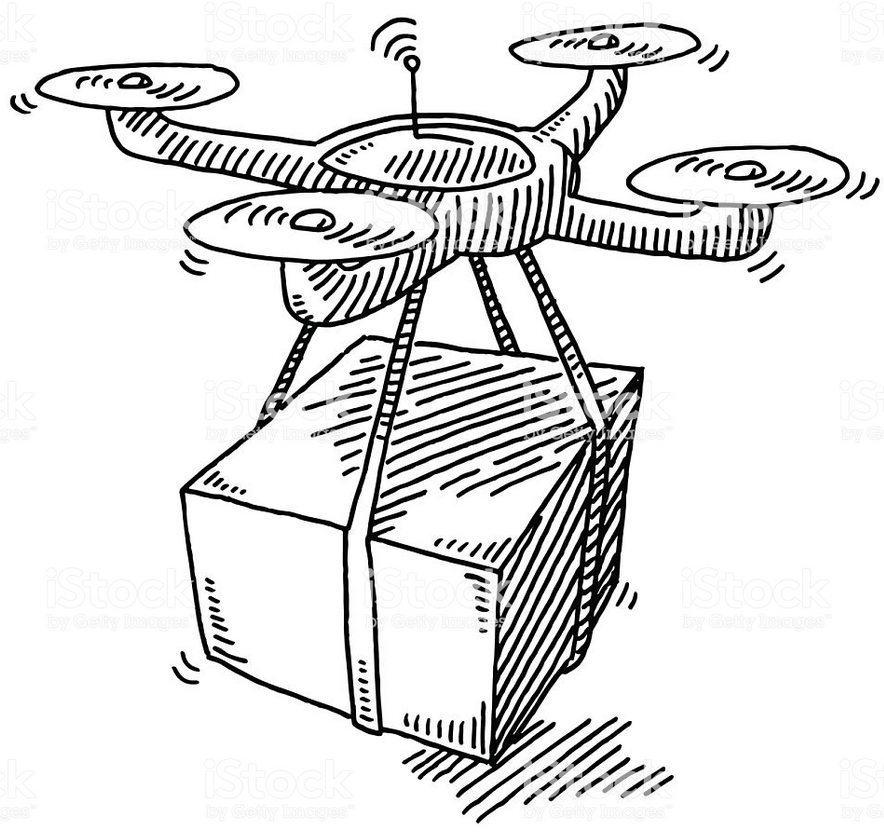
\includegraphics[width=0.22\textwidth]{img/amazon.png}
\end{wrapfigure}

Početkom ove godine američka tvrtka Amazon pokreće projekt \textit{Amazon
Prime Air}.  To znači da ćete moći naručiti paket s Amazona, a njega će vam
dostaviti dron u roku od $30$ minuta.

Svaki dron u skladištu ima u redu svojih $M$ paketa koje mora dostaviti tim
redoslijedom kako su poredani. Za svaki paket znamo njegovu masu $K_i$,
izraženu u kilogramima. Dron u jednoj dostavi može prenijeti najviše $N$
kilograma paketa i može ponijeti više uzastopnih paketa odjednom (počevši od
prvog u redu). Naravno, zbroj kilograma ponesenih uzastopnih paketa mora biti
manji ili jednak $N$.

Amazon želi optimizirati broj polijetanja te ih zanima u koliko najmanje
polijetanja dron može prenijeti pakete na zadana odredišta. Nažalost, oni to
ne znaju izračunati pa su zamolili vas da to učinite umjesto njih.

%%%%%%%%%%%%%%%%%%%%%%%%%%%%%%%%%%%%%%%%%%%%%%%%%%%%%%%%%%%%%%%%%%%%%%
% Input
\subsection*{Ulazni podaci}
U prvom je retku prirodan broj $N$ $(1 \le N \le 100)$ iz teksta zadatka.

U drugom je retku prirodan broj $M$ $(1 \le M \le 100)$ iz teksta zadatka.

U sljedećih $M$ redaka nalazi se po jedan broj $K_i$ $(1 \le K_i \le N)$
koji označava masu $i$-tog paketa.

%%%%%%%%%%%%%%%%%%%%%%%%%%%%%%%%%%%%%%%%%%%%%%%%%%%%%%%%%%%%%%%%%%%%%%
% Output
\subsection*{Izlazni podaci}
Ispišite minimalan broj polijetanja drona.

%%%%%%%%%%%%%%%%%%%%%%%%%%%%%%%%%%%%%%%%%%%%%%%%%%%%%%%%%%%%%%%%%%%%%%
% Scoring
\subsection*{Bodovanje}
U testnim primjerima vrijednima $10$ bodova, vrijedit će $M=3$.
U testnim primjerima vrijednima dodatnih $10$ bodova, vrijedit će da su svi
paketi jednake mase.

%%%%%%%%%%%%%%%%%%%%%%%%%%%%%%%%%%%%%%%%%%%%%%%%%%%%%%%%%%%%%%%%%%%%%%
% Examples
\subsection*{Probni primjeri}
\begin{tabularx}{\textwidth}{X'X'X}
\sampleinputs{test/amazon.dummy.in.1}{test/amazon.dummy.out.1} &
\sampleinputs{test/amazon.dummy.in.2}{test/amazon.dummy.out.2} &
\sampleinputs{test/amazon.dummy.in.3}{test/amazon.dummy.out.3}
\end{tabularx}

\textbf{Pojašnjenje trećeg probnog primjera:}
Optimalno je uzeti prvi paket u prvoj dostavi, a drugi i treći paket u drugoj
dostavi.

%%%%%%%%%%%%%%%%%%%%%%%%%%%%%%%%%%%%%%%%%%%%%%%%%%%%%%%%%%%%%%%%%%%%%%
% We're done
\end{statement}

%%% Local Variables:
%%% mode: latex
%%% mode: flyspell
%%% ispell-local-dictionary: "croatian"
%%% TeX-master: "../hio.tex"
%%% End:
